\documentclass[ngerman]{article}

%\NeedsTeXFormat{LaTeX2e}
\usepackage[utf8]{inputenc}
\usepackage[german]{babel}
%\usepackage{ngerman}
\usepackage{hyperref}
\usepackage{hhline}
\usepackage{varioref}
\usepackage[table]{xcolor}
\usepackage{graphicx}
\usepackage{float}
\usepackage{amssymb}
\usepackage{amsmath}

\usepackage[
        hyperref=true,          % Klickbare Referenzen in der PDF-Datei
        backref=true,           % In der Literaturref. die Seiten angeben, wo ein \cite dazu steht
        bibencoding=inputenc,   % s. inputenc-Paket
        style=numeric,
        backend=bibtex,
        sorting=nty]{biblatex}  % http://dante.ctan.org/tex-archive/help/Catalogue/entries/biblatex.html
\renewcommand{\mkbibnamelast}[1]{\textsc{#1}}
\bibliography{ausarbeitung}

\author{Sebastian Bernauer}
\title{NP-Vollständigkeit wichtiger Probleme}
\date{22.03.2019}

\begin{document}

\maketitle
\tableofcontents
\newpage

\listoffigures
\listoftables
\newpage

\section{Komplexitätsklassen}
Probleme in der Informatik werden Probleme in verschiedene Komplexitätsklassen aufgeteilt.\\
Der Operator $L_1\ \le_p L_2$ bedeutet, dass das $L_1$ polynomiell auf $L_2$ reduzierbar ist.
Dies ist der Fall, wenn es eine polynomielle Transformation von $L_1$ nach $L_2$ gibt, so das heißt, wenn es eine von einer DTM in polynomieller Zeit berechenbare Funktion $f: \sum_1^* \rightarrow \sum_2^*$ gibt, so dass für alle $w \in \sum_1^*$ gilt:
$$w \in L_1 \leftrightarrow f(w) \in L_2$$
Dieser Operator $\le_p$ kann nun Probleme in diverse Problemklassen einteilen.
In der Tabelle \vref{tab:Problemklassen} sind häufige Problemklassen dargestellt.

\begin{table}[H]
	\centering
	\begin{tabular}{ | p{3,5cm} | p{7,5cm} | }
		\hline \rowcolor{gray!15}
		\textbf{Komplexitätsklasse} & \textbf{Beschreibung} \\ \hhline{|=|=|}
		P & Polynomiell lösbar \\ \hline
		NP & Nichtdeterministisch polynomiell lösbar \\ \hline
		NP-vollständig & Schwierigste Probleme in NP \\ \hline
		NP-schwierig & Genauso schwer wie NP-vollständig, das Problem muss aber nicht in NP enthalten sein\\ \hline
		nicht rekursiv & Sehr, sehr schwere Probleme\\ \hline	
	\end{tabular}
	\caption{Häufige Problemklassen}
	\label{tab:Problemklassen}
\end{table}

\subsection{NP-vollständig}
Ein Problem/Sprache L ist NP-vollständig, wenn folgendes gilt:\\
\begin{itemize}
\item $L \in NP$
\item $\forall L` \in NP: L` \leq_p L$
\end{itemize}

\subsection{NP-schwierig}
Ein Problem/Sprache L ist NP-schwierig, wenn folgendes gilt:\\
\begin{itemize}
\item $\forall L` \in NP: L` \leq_p L$
\end{itemize}

\section{Satisfiability Problem (SAT)}
\subsection{Problembeschreibung}
Für natürliche Zahlen \(n\) und \(m\) seien \(m\) Klauseln über \(n\) Variablen gegeben.
Eine Klausel ist die Disjunktion [Veroderung] von einigen Literalen \(x_i\) bzw. \(\overline{x_i}\) mit \(i,j \in \{1,...,n\}\). Es soll entschieden werden, ob es eine Belegung \(a = \{a_1,...,a_n\} \in \{0,1\}^n\) der Variablen \(x_1,...,x_n\) gibt, so dass alle Klauseln erfüllt sind.\\
Eine mögliche Fragestellung für das SAT-Problem ist: Existiert eine Wahrheitsbelegung der Variablen \(x_1,...,x_n\), so dass alle Klauseln erfüllt sind?\\
Der Beweis, dass das SAT-Problem ist der Satz von Cook, der in der vorherigen Präsentation gezeigt wurde. Er ist unter \cite{wegener} in dem Kapitel 3.3.7 zu finden.
\subsection{3-SAT}
3-SAT ist ein Spezialfall von SAT, bei denen jede Klausel die Länge 3 hat, also 2 Literale besitzt.
Im Folgenden wird bewiesen, dass das allgemeine SAT-Problem durch das 3-SAT Problem abbildbar ist.
Durch den Beweis wird gezeigt, dass die zwei Probleme gleich komplex und somit beide NP-vollständig sind (SAT wurde ja durch den Satz von Cook als NP-vollständig bewiesen).
\subsection{Beweis: SAT $\le_p$ 3-SAT}
Das grundsätzliche Vorgehen, um SAT-Probleme in 3-SAT-Probleme abzubilden ist, alle Klauseln in neue Klauseln der Länge 3 zu überführen.
Haben die ursprüngliche, allgemeinen Klauseln die Länge $\le$ 3, sind die Umformungen trivial:
\begin{itemize}
\item Länge 1: Die Klausel besteht aus einem Literal $z$\\
Neue Klausel der Länge 3: $z \vee z \vee z$\\
Durch die Umformung wird die semantische Bedeutung der Klausel nicht verändert, dies könnte z.B. durch eine Wahrheitstabelle bewiesen werden.
\item Länge 2: Die Klausel besteht aus 2 Literalen $z \vee y$\\
Neue Klausel: $z \vee z \vee y$\\
Hier gilt das Gleiche wie bei der Umformung einer Klausel der Länge 1.
\item Länge 3: Die Klausel besteht aus 3 Literalen $z \vee y \vee z$\\
Neue Klausel: $z \vee y \vee z$\\
An dieser Stelle besteht die Klausel bereits aus 3 Literalen, es muss keine Umformung durchgeführt werden.
\end{itemize}
Hat die ursprüngliche Klausel eine Länge $\ge$ 4, wird die Umformung schwieriger.
Hier wird für das Verständnis zunächst eine beispielhafte Umformung gezeigt, anschließend wird die allgemeine Umformung definiert.\\
Beispiel: Klausel der Länge $k = 7$ mit den Literalen $z_1 \vee ... \vee z_k$ wird umgeformt zu folgenden 5 Klauseln der Länge 3:
\begin{enumerate}
\item $z_1 \vee z_2 \vee y_1$
\item $\overline{y_1} \vee z_3 \vee y_2$
\item $\overline{y_2} \vee z_4 \vee y_3$
\item $\overline{y_3} \vee z_5 \vee y_4$
\item $\overline{y_4} \vee z_6 \vee z_7$
\end{enumerate}
Die Literale $y_1, ..., y_4$ sind eingeführte ``Hilfsvariablen'' und werden benötigt, um die Klausel aufzutrennen ohne die Bedeutung zu verändern.
Betrachten wir die entstandene Klausel 3:
Es ist zu erkennen, dass durch das Literal $\overline{y_2}$ entweder die vorherige Klausel (2) oder die aktuelle Klausel (3) erfüllt werden muss.
Dies entspricht dem Operator, der in der ursprünglichen Klausel zwischen den Literalen stand, dem logischen ODER.
Das zweite Literal in der neuen Klausel - $z_5$ - wurde von der ursprünglichen Klausel übernommen.
Mit dem dritten und letztem Literal $y_4$ wurde die ODER-Verknüpfung zu der nächsten entstandenen Klausel geschaffen.\\
Das war ein konkretes Beispiel, um eine Klausel der Länge $k=7$ in Klauseln der Länge 3 zu überführen.
Die allgemeine Umformung für Klauseln der Länge $k\ge4$ sieht wie folgt aus:
$c$ ist die Nummer der Klausel und wurde eingeführt, um die Hilfsvariablen der Klauseln formal zu trennen.
\begin{enumerate}
\item $z_1 \vee z_2 \vee y_{c,1}$
\item $\overline{y_{c,l}} \vee z_{l+2} \vee y_{c,l+1}$ für $1 \le l \le k - 4$
\item $\overline{y_{c,k-3}} \vee z_{k-1} \vee z_k$
\end{enumerate}
Das Prinzip bleibt das Gleiche, wie bei dem Beispiel mit $k=7$, die Umformung ist nur allgemein definiert.\\
Durch die Transformation eines SAT-Problem in ein 3-SAT-Problem wurde bewiesen, dass das 3-SAT-Problem NP-vollständig ist.

\section{Clique Problem}
\subsection{Problemstellung}
In einem ungerichteten Graphen $G = (V,E)$ bildet die Knotenmenge $V` \subseteq V$ eine Clique, wenn für alle $v, v` \in V`$ gilt: $${v,v`} \in E$$
In den Abbildungen \vref{fig:Clique3} und \vref{fig:Clique4} sind 2 Graphen mit Cliquen dargestellt.

\begin{figure}[H]
	\centering
	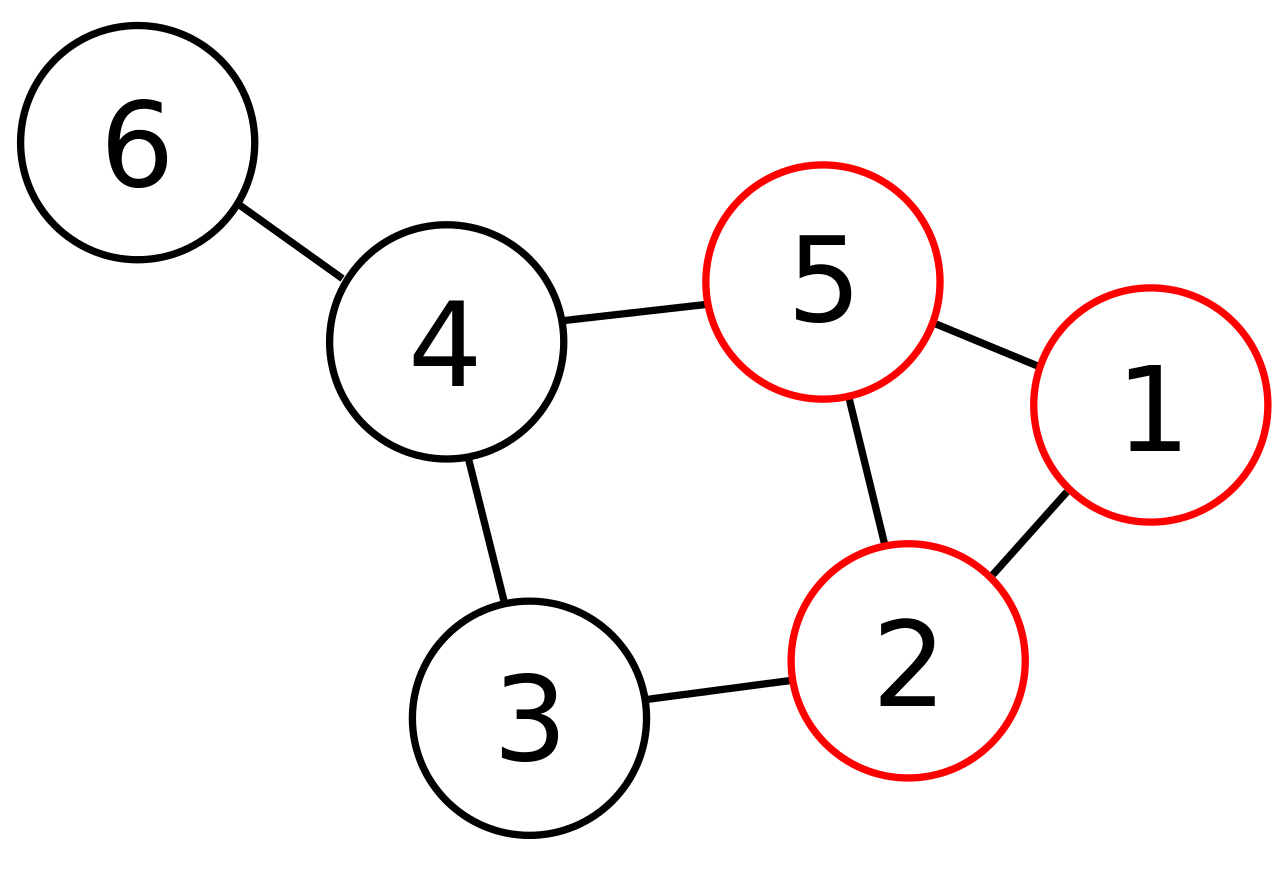
\includegraphics[width=4cm]{figures/clique1.png}
	\caption[Ein Graph mit einer Clique der Größe 3]{Ein Graph mit einer Clique der Größe 3. Bildquelle: \cite{cliqueImage1}}
	\label{fig:Clique3}
\end{figure}

\begin{figure}[H]
	\centering
	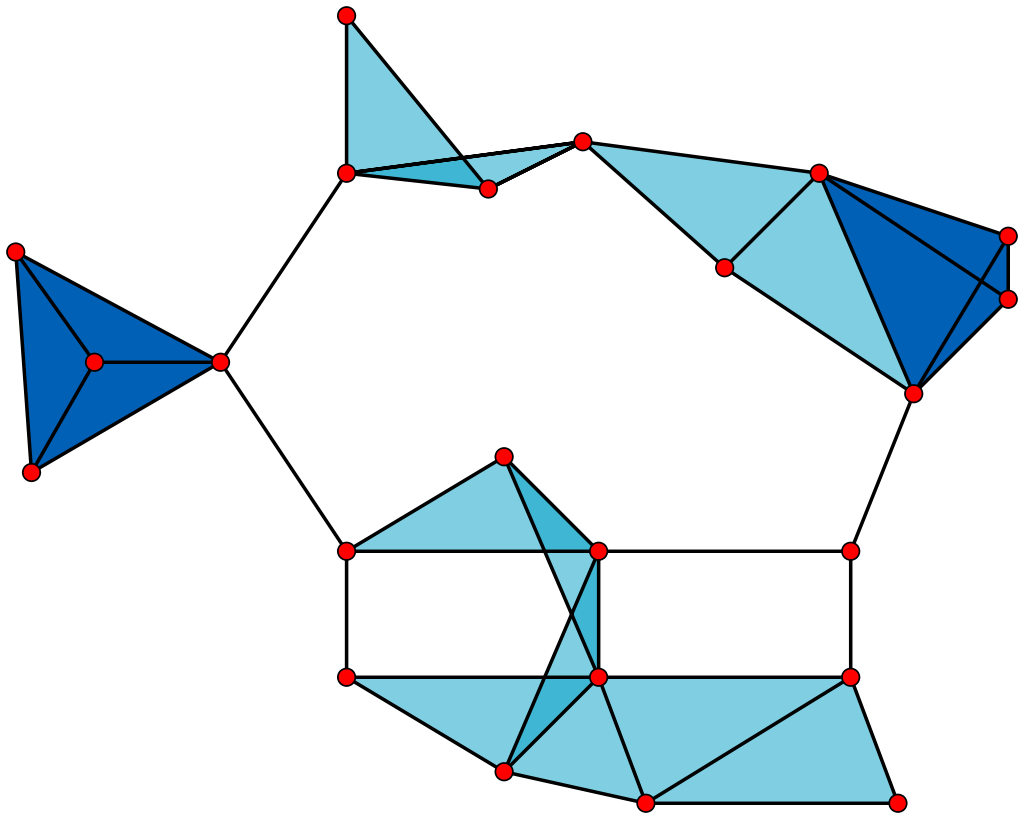
\includegraphics[width=5cm]{figures/clique2.png}
	\caption[Ein Graph mit zwei Cliquen der Größe 4]{Ein Graph mit zwei Cliquen der Größe 4 (dunkelblau) und vielen Cliquen der Größe 3 (türkis). Bildquelle: \cite{cliqueImage2}}
	\label{fig:Clique4}
\end{figure}

\subsection{Fragestellungen}
Es gibt für die meisten Probleme 3 Fragestellungen, diese sind in Tabelle \vref{tab:Fragestellungen} aufgeführt.
\begin{table}[H]
	\centering
	\begin{tabular}{ | p{3,5cm} | p{7,5cm} | }
		\hline \rowcolor{gray!15}
		\textbf{Fragestellung} & \textbf{Beschreibung} \\ \hhline{|=|=|}
		Entscheidungsproblem & Liefert wahr oder falsch \\ \hline
		Werteproblem & Liefert eine Zahl \\ \hline
		Optimierungsproblem & Liefert die Lösung des Problems, z.B. eine Menge an Knoten \\ \hline	
	\end{tabular}
	\caption{Die 3 Fragestellungen bei Problemen}
	\label{tab:Fragestellungen}
\end{table}
Für das Clique-Problem gibt es die folgenden 3 Fragestellungen:
\begin{enumerate}
\item \textbf{Entscheidungsproblem}: Gibt es eine Clique der Größe k?\\
\item \textbf{Werteproblem}: Berechne das größte k, so dass eine Clique der Größe k vorhanden ist.\\
\item \textbf{Optimierungsproblem}: Berechne eine Clique mit dem größten k.\\
\end{enumerate}

\subsection{Beweis: Clique ist NP-vollständig}
Der Bewies, dass Clique NP-vollständig ist, teilt sich in 2 Teile auf:
\begin{enumerate}
\item Clique ist in NP enthalten
\item SAT $\le_p$ Clique
\end{enumerate}
Die Beweise werden in den nächsten 2 Kapiteln durchgeführt.

\subsubsection{Beweis: Clique ist in NP enthalten}
Das Clique-Problem kann mit einer NTM gelöst werden. Dies geht wie folgt vor:
\begin{enumerate}
\item NTM zählt Anzahl $n$ der Knoten im Graphen
\item Rät Wort $w \in \{0,1\}^n$
\item Das Wort wird als Knotenauswahl interpretiert, $V'$ enthält alle Knoten $i$ mit $w_i = 1$
\item Es wird getestet, ob
\begin{enumerate}
\item \(V'\) genau \(k\) Knoten beinhaltet.
\item \(G\) eine Clique auf \(V'\) enthält
\end{enumerate}
\end{enumerate}
Der Rechenaufwand hierfür ist polynomiell in der Knotenzahl $n$.
Es wurde bereits bewiesen, dass NTM durch DTM abgebildet werden können.
Die polynomielle Laufzeit des Entscheidens, die angegebenen Knoten eine Clique bilden, kombiniert mit dem Nichtdeterminismus ergibt die Problemklasse NP für das Cliquen-Problem.

\subsubsection{Beweis: SAT $\le_p$ Clique}
\label{sec:SAT_Clique}
Konstruiere einen Graphen, der mittels \(Clique\) ein Problem löst, welches ein \(SAT\)-Problem ist.
Dadurch wird das SAT-Problem in ein Clique-Problem transferiert.
\begin{enumerate}
\item Füge für jedes Literal in den Klauseln einen Knoten hinzu.
\item Verbinde alle Literale außer folgende Kanten:
\begin{itemize}
\item Klauselgruppen untereinander
\item Gegensätzliche Literale (z.B. \(x_1\) und \(\overline{x_1}\))
\end{itemize}
\item Suche eine Clique der Größe k, k ist die Anzahl der Klauseln.
Da die Knoten einer Klauselgruppe nicht verbunden sind, muss aus jeder Klausel ein Literal ``wahr'' sein.
Da die Literale in den Klauseln ODER-verknüpft sind, sind alle Klauseln erfüllt.\\
\end{enumerate}
In Abbildung \vref{fig:Clique_Sat} ist ein beispielhaftes SAT-Problem als Clique-Graph dargestellt.
Der Graph wurde nach den oben genannten Regeln erstellt.
Der Beweis wurde \cite{weitz} entnommen.\\
Die Transformation von SAT in Clique (Schritte 1 + 2) findet in polynomieller Zeit statt, weshalb gilt: SAT $\le_p$ Clique.\\
Damit ist bewiesen: Clique ist NP-vollständig.
\begin{figure}[H]
	\centering
	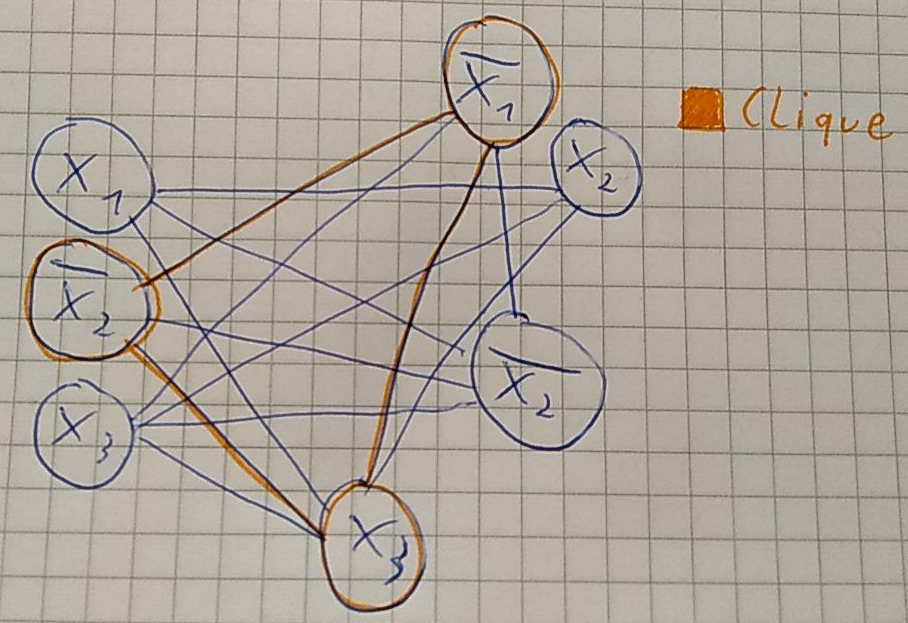
\includegraphics[width=7cm]{figures/clique_sat.png}
	\caption{Beispielhafte Darstellung SAT-Problem als Clique-Problem}
	\label{fig:Clique_Sat}
\end{figure}

\section{Knapsack Problem (KP)}
\subsection{Problemstellung}
Gegeben sind ein Rucksack und \(n\) Objekte mit Gewichten \(g_1,...,g_n \in \mathbb{N}\) sowie eine Gewichtsschranke $G$.
Zusätzlich seien \(a_1,...,a_n \in \mathbb{N}\) die Nutzenwerte für die Objekte.\\
Eine grafische Darstellung eines Knapsack Problems ist in Abbildung \vref{fig:Knapsack} abgebildet.

\begin{figure}[H]
	\centering
	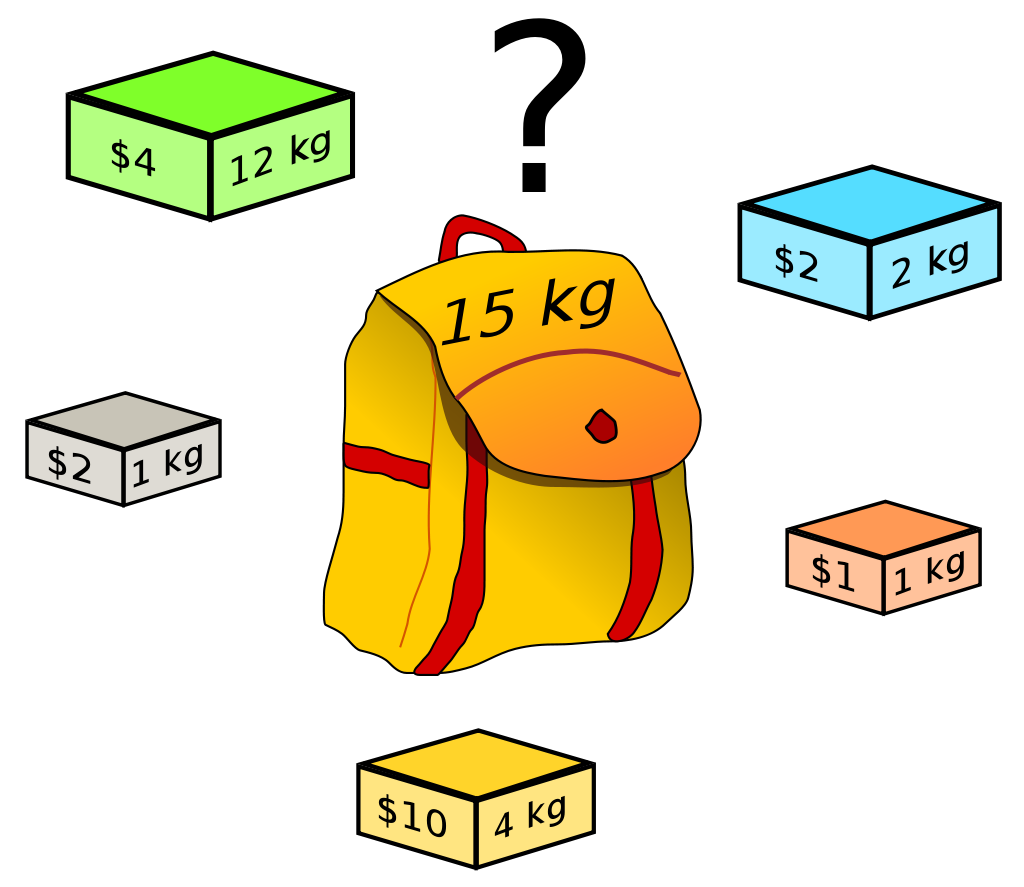
\includegraphics[width=5cm]{figures/knapsack.png}
	\caption[Grafische Darstellung eines Knapsack Problems]{Grafische Darstellung eines Knapsack Problems. Bildquelle: \cite{knapSackImage1}}
	\label{fig:Knapsacks}
\end{figure}

\subsection{Fragestellungen}
Bei dem KP-Problem gibt es die folgenden 3 Fragestellungen:
\begin{enumerate}
\item \textbf{Entscheidungsproblem}: Gibt es - unter Beachtung des Gewichtslimits - eine Beladung mit mindestens diesem Nutzwert?\\
\item \textbf{Werteproblem}: Berechne den größtmöglichen Nutzwert x.\\
\item \textbf{Optimierungsproblem}: Berechne die optimale Beladung.\\
\end{enumerate}

\subsection{KP ist NP-vollständig}
\label{sec:BeweisKP}
Der Beweis sei an dieser Stelle vorausgesetzt.
Es wird bewiesen, dass 3-SAT \(\le_p\) KP ist.\\
Für Interessierte ist er unter \cite{wegener} im Kapitel 3.4.3 auf Seite 55 zu finden.
Der Beweis, dass KP NP-vollständig ist wichtig, da in dem nächsten Beweis darauf aufgebaut wird.

\section{Partition Problem}
\subsection{Problemstellung}
Gegeben sind \(b_1,...,b_n \in \mathbb{N}\). Gibt es eine Teilmenge \(I \subseteq \{1,...,n\}\), so dass die Summe aller \(b_i, i \in I\) gleich der Summe aller \(b_i, i \notin I\) ist?
Umgangssprachlich wir versucht, eine Menge von Gewichten in 2 gleich schwere Haufen aufzuteilen.

\subsection{Beweis: Partition ist NP-vollständig}
Es wurde bereits bewiesen, dass ein (spezielles) Knapsack Problem \(KP\mbox{*}\) NP-vollständig ist. (siehe Kapitel \vref{sec:BeweisKP})\\
(Für \(a_1,...,a_n\) soll entschieden werden, ob es eine Auswahl gibt, so dass die Summe genau \(A\) beträgt).\\
Nun ist zu beweisen, dass \(KP\mbox{*} \leq_p PARTITION\).\\
Daraus würde folgen, dass $PARTITION$ NP-vollständig ist.\\
Sei \((a_1,...,a_n,A)\) eine Eingabe für \(KP\mbox{*}\).\\
Daraus konstruieren wir in polynomieller Zeit die Eingabe\\
\((a_1,...,a_n,S-A+1,A+1)\) für \(PARTITION\), wobei \(S\) die Summe aller \(a_i\) ist.\\
Falls \(I\) eine Lösung für das \(KP\) ist, erhalten wir mit \(I \cup \{n+1\}\) eine Lösung für \(PARTITION\), da\\
$$\sum_{i \in I}a_i + S - A + 1 = S + 1 = \sum_{1 \le i \le n}a_i + 1 = \sum_{i \notin I}a_i + A + 1$$\\
Sie Summe aller Zahlen in der Eingabe für \(PARTITION\) beträgt \(2S + 2\).
Ein Lösung für \(PARTITION\) muss also so aussehen, dass jeder Teil sich zu \(S + 1\) aufsummiert.
Damit müssen die Zahlen \(S - A + 1\) und \(A + 1\) in verschiedenen Teilen sein.
\((S - A + 1) + (A + 1) = (S + 2) > (S + 1)\)
Die Zahlen, die \(S - A + 1\) zu \(S + 1\) ergänzen, haben die Summe \(A\) und bilden eine Lösung für die Eingabe von \(KP\mbox{*}\).
Der Beweis wurde \cite{wegener} entnommen.\\
Damit wurde bewiesen: Partition ist NP-vollständig.

\section{Zusammenfassung}
Alle behandelten Probleme - SAT, Clique, KP und Partition waren NP-vollständig.
Als ersten Problem wurde mit dem Satz von Cook das SAT-Problem als NP-vollständig bewiesen.
Darauf aufbauend wurde das 3-SAT, Clique, KP und Partition-Problem bewiesen.
Es ist klar erkennbar, wie die Beweise aufeinander aufbauen, und einem so komplexe Beweise wie der Satz von Cook erspart werden, da auf dem Satz aufgebaut werden kann.\\
Alle genannten Probleme sind NP-vollständig, somit gelten folgende Bedingungen für sie:
\begin{enumerate}
\item $L \in NP$
\item $\forall L` \in NP: L` \leq_p L$
\end{enumerate}
Aus der zweiten Bedingung folgert, dass die Probleme (in polynomieller Zeit) in einander umgewandelt werden können.
Besonders anschaulich passiert dies bei der Umwandlung des SAT in das Clique-Problem in Kapitel \vref{sec:SAT_Clique}.

\newpage
\def\refname{Literaturverzeichnis}
\printbibliography

\end{document} 
